\section{Experimental setup and Procedure}
\label{sec:procedure}
In order to derive the magnetic moments and gyromagnetic ratios, 
we use the relationship to applied magnetic fields given by the Zeeman effect 
as established in the theory section \ref{sec:theory)}. 
The point of resonance leads to the appearance of absorption lines 
in the strength of the highly oscillating field. These absorption lines 
will then be measured. 
The steps undertaken in this experiment are the following:
\begin{enumerate}
\item
measuring the homogenity of the magnetic field in order to define a stable working point;
\item
measuring the resonance frequency for a given external magnetic field by searching for 
equidistant absorption peaks;
\item
measuring the resonance frequency with a lock-in amplifier and sine modulated saw tooth signal.
\end{enumerate}
From the obtained data, we then calculate the following quantities:
\begin{enumerate}
\item
nuclear magnetic moment of $^19$F;
\item
gyromagnetic moment of proton in $^1$H, glycole and fluor.
\end{enumerate}

\begin{figure}[htpb]
    \centering
    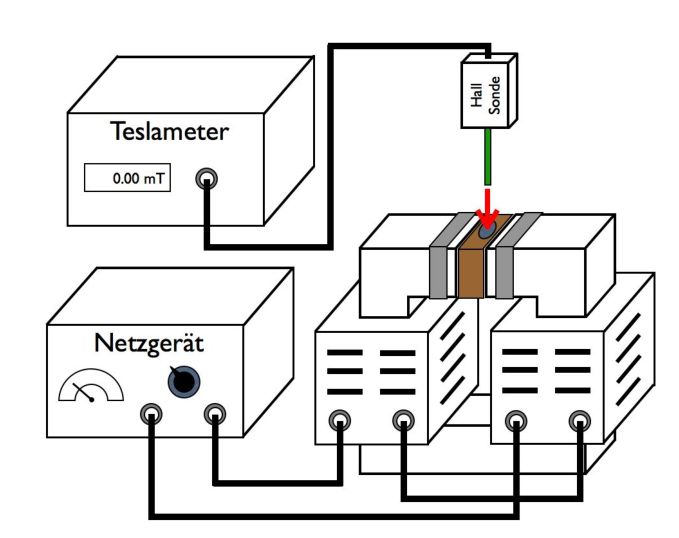
\includegraphics[width=0.8\linewidth]{figures/setup1}
    \caption{\textbf{Step 1:} Measuring the magnetic field with the help of 
       an hall effect sensor. As you can notice from the figure we 
      apply various Potentials, which cause an current in the coil which
      further results in an magnetic field sensing by the hall effect sensor \cite{versuchsanleitung}.}
    \label{fig:figures/setup1}
\end{figure}
\begin{figure}[htpb]
    \centering
    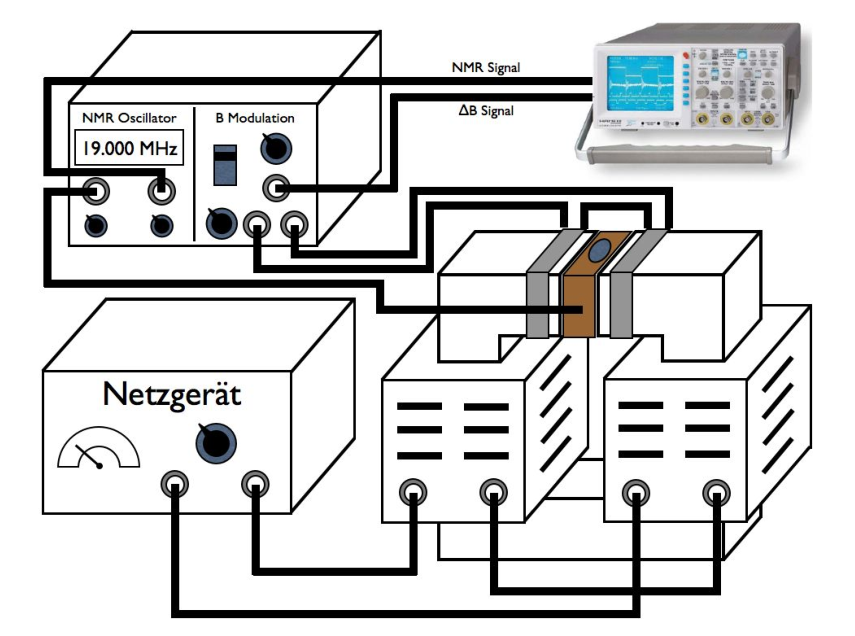
\includegraphics[width=0.8\linewidth]{figures/setup2}
    \caption{\textbf{Step 2:} Measuring the resonance frequency with the first
        method. You notice that we do not use the lockin aplifier yet,
        this will be the case in the following steps, instead we vary the
        frequency with constant current and voltage in oder to observe
        the periodic peaks as already described.}
    \label{fig:figures/setup1}
\end{figure}
\begin{figure}[htpb]
    \centering
    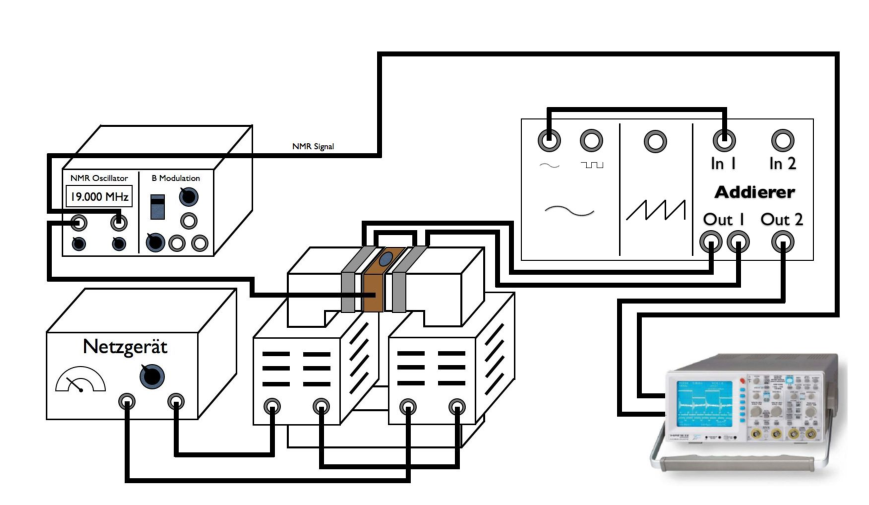
\includegraphics[width=0.8\linewidth]{figures/setup3}
    \caption{\textbf{Step 3:}
        We used this experimental setup to calibrate the following
        measurement with the lockin method.}
    \label{fig:figures/setup1}
\end{figure}
\begin{figure}[htpb]
    \centering
    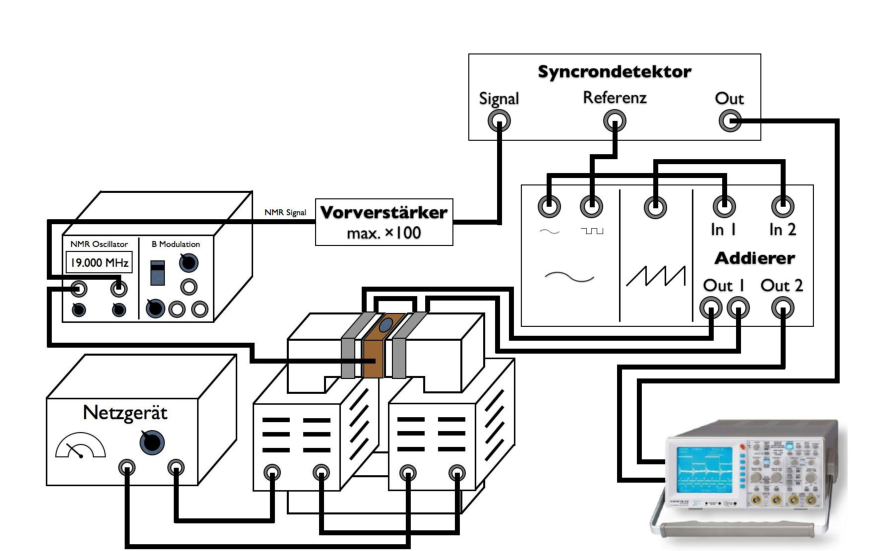
\includegraphics[width=0.8\linewidth]{figures/setup4}
    \caption{\textbf{Step 4:}
        Finally we can use this experimental setup to measure
        the resonance frequency with the lockin method.}

    \label{fig:figures/setup1}
\end{figure}
\clearpage




